\documentclass[a4paper,10pt]{article}
%\documentclass[a4paper,10pt]{scrartcl}

\usepackage[utf8]{inputenc}
%\usepackage{listings}
\usepackage{tikz}

\usetikzlibrary{arrows,automata}


\title{TP3 ACT}
\author{Matthieu Caron et Armand Bour}
\date{vendredi 9 octobre 2015}

\pdfinfo{%
  /Title    (TP2 ACT)
  /Author   (Matthieu Caron et Armand Bour)
  /Creator  (Matthieu Caron et Armand Bour)
  %/Producer ()
  %/Subject  ()
  %/Keywords ()
}

\begin{document}
\maketitle

\paragraph{Question 1}

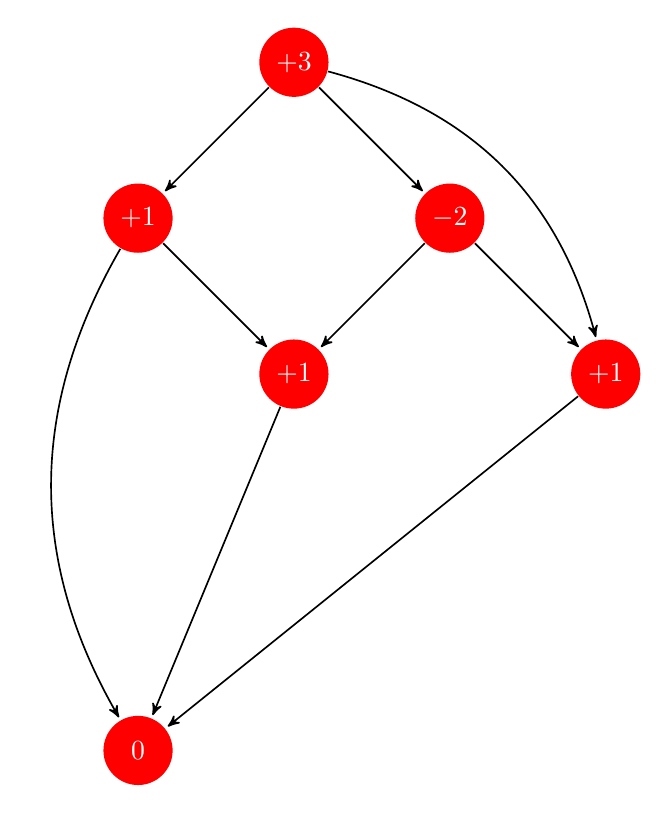
\begin{tikzpicture}[->,>=stealth',shorten >=1pt,auto,node distance=2.8cm,semithick]
    \tikzstyle{every state}=[fill=red,draw=none,text=white]

    \node[state] (A) {$+3$};
    \node[state] (B)[below left of=A] {$+1$};
    \node[state] (C)[below right of=A] {$-2$};
    \node[state] (D)[below left of=C] {$+1$};
    \node[state] (E)[below right of=C] {$+1$};
    \node[state] (F)[below of=D][below left of=E][below right of=B] {$0$};

    \path (A) edge              node {} (B)
    (B) edge                  node {} (D)
    (A) edge              node {} (C)
    (C) edge              node {} (D)
    (C) edge          node {} (E)
    (A) edge [bend left]         node {} (E)
    (B) edge [bend right]        node {} (F)
    (E) edge                     node {} (F)
    (D) edge                     node {} (F);
\end{tikzpicture}


\paragraph{Question 2}
S’ils sont tous positifs : $res = -1 * min(successeurs)-1$\newline
Sinon : $res = -1*max(desValeursNegatives) + 1$

\paragraph{Question 3}
La fonction récursive $naif$ calcule toutes les sous-tablettes possibles. Quatre boucles sont utilisées, une pour chaque possibilité de cassure (x colonne(s) à gauche ou à droite, et x ligne(s) en haut ou en bas). Des possibilités sont alors calculées plusieurs fois.\newline
En Python, la fonction prends en temps respectivement pour les configurations suivantes :
\begin{description}
\item[(10, 7, 7, 3)] 4 minutes 47 secondes ;
\item[(10, 7, 5, 3)] 10 minutes 24 secondes.
\end{description}

La différence de temps est due à la “profondeur” de la tête de mort dans la tablette. Dans le second cas, elle est plus proche du centre, ce qui décuple le nombre de sous-arbres possiblites.\newline
La complexité est exponentielle % TODO: justifier %

\paragraph{Question 4}


\paragraph{Question 5}







\end{document}
